\chapter{DFR-FastMOT: Detection Failure Resistant Tracker for Fast  Multi-Object Tracking Based on Sensor Fusion(ICRA2023)\cite{10160328}}

\section{解决问题}
文章主要针对目标追踪中的遮挡问题做了许多工作。
非学习算法往往只保存一小段的轨迹,因此难以应对长时间的遮挡情况。
文章设计了一种代数的数据关联公式从而降低了需要计算复杂度,从而可以处理更长时间的轨迹。

\section{解决算法}
\begin{figure}[htbp]
	\centering
	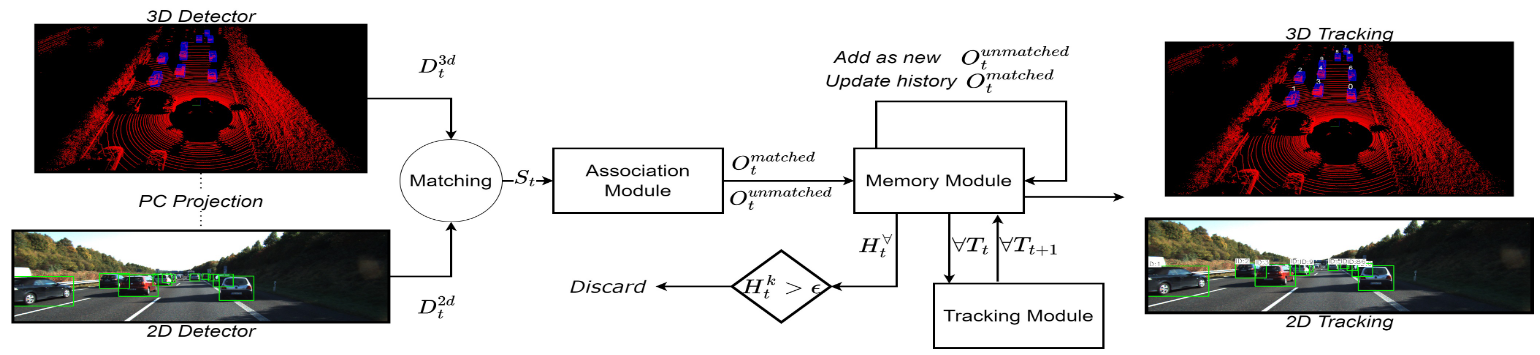
\includegraphics[width=\textwidth]{images/DFRMOT/framework.png}
	\caption{整体框架}
	\label{framework}
\end{figure}

\subsection{关联矩阵的引入}
为了提高计算的效率,文章为每种传感器设计了一个关联矩阵,矩阵的每个元素代表前一时刻对象(轨迹)的估计值和当前时刻检测值的关联程度。

\begin{figure}[H]
	\centering
	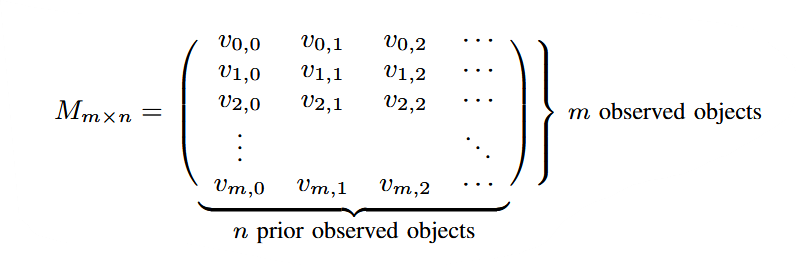
\includegraphics[width=0.8\textwidth]{images/DFRMOT/matrix.png}
\end{figure}

\begin{tcolorbox}[]

\hspace{22pt}$v_{i,j}$代表关联值,公式\ref{equ_0}处理2D情况,记作$M_c$。公式\ref{equ_1}处理3D情况,记作$M_l$。公式\ref{equ_2}将两种情况进行统一,记作$M_f$。

\begin{equation}\label{equ_0}
	v_{ij} = 
	\begin{cases}
		v_{IoU}&:v_{IoU}\leq a_c\\
		0&:\text{Otherwise}.
	\end{cases}
\end{equation}

\begin{equation}\label{equ_1}
	v_{ij} = 
	\begin{cases}
		v_{dist} & :v_{dist} < a_l\\
		a_l & :\text{Otherwise}.
	\end{cases}
\end{equation}

\begin{equation} \label{equ_2}
\begin{cases}
	M_f &= \alpha_c M_c + \alpha (1 - M_t), \\
	\alpha_c + \alpha_l &= 1, \\
	\alpha_c , \alpha_l &\leq 1.
\end{cases}
\end{equation}

\hspace{22pt}得到所有关联矩阵之后,便可以进行数据关联。文章采用了类匈牙利算法来实现该步骤。
最后所有的计算复杂度为:
$$ \mathcal{O}(2mn) \rightarrow \mathcal{O}(m^2n^2) \rightarrow \mathcal{O}(m^2n^2) $$

\end{tcolorbox}

\subsection{其它处理方法}
1. 3D距离函数的选用

为了处理遮挡的情况,文章采用了3D中心距离来衡量两个目标的相似程度,而不是传统的IoU。当出现长时间的遮挡情况时,去计算IoU是十分困难的,而计算3D的距离则更容易实现。

2. KF计算简化

在用KF计算目标下一时刻的状态时,需要进行大量的矩阵运算。为此,作者采用最少点数来描述目标位置:2D两个,3D两个。

\section{文章结果}
文章通过使用不同质量的检测器来模拟遮挡的效果。结果表明,文章显著提高了低质量检测器的追踪效果。整体而言,追踪的精度也有所提高。
\begin{figure}
	\centering
	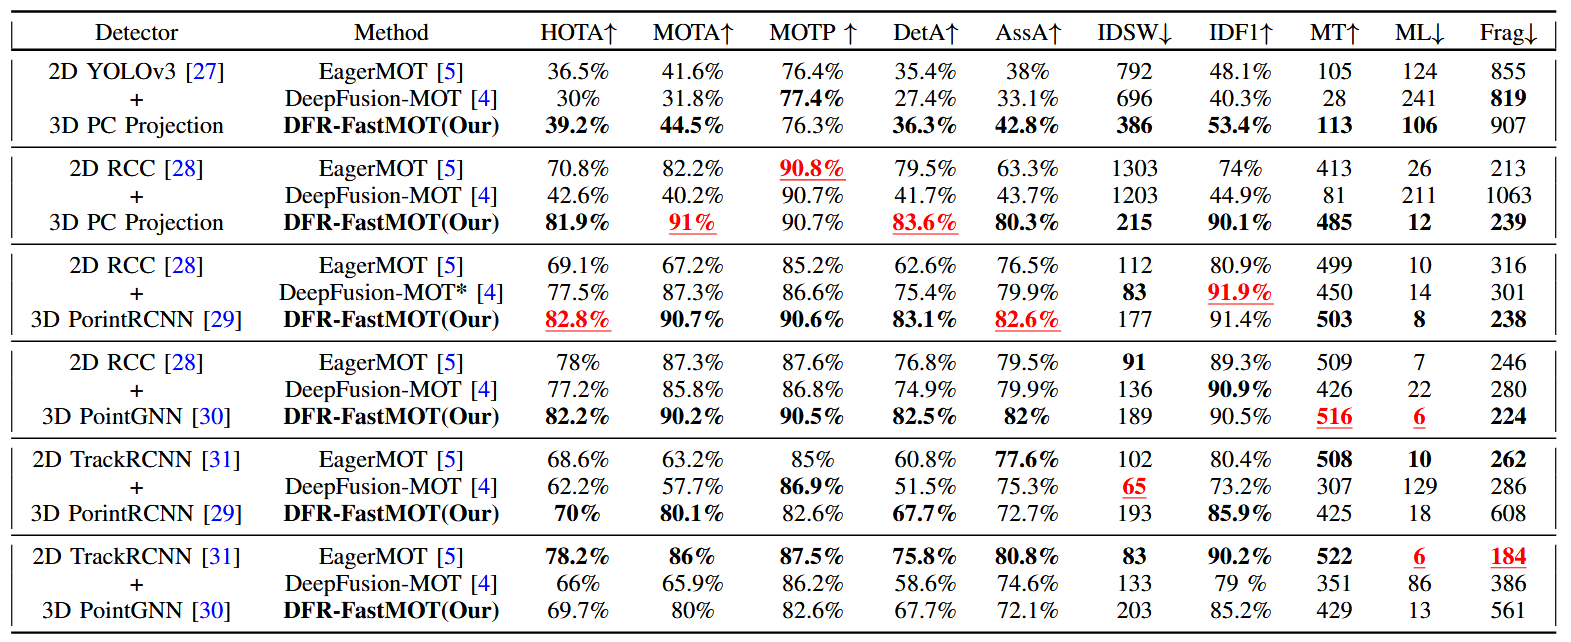
\includegraphics[width=\textwidth]{images/DFRMOT/result.png}
\end{figure}


\section{学习总结}
DFRMOT也是采用DBT追踪框架,具体内容也基本和EagerMOT相似。其主要工作在于提出了一种提高计算效率的关联矩阵,由此多出的冗余可以用来计算更长时间的目标,间接的提高了应对遮挡的能力。

所以,在自己设计的追踪器上,就可以采用本文设计的关联矩阵提高计算效率。
此外,本外还在细节上提出了许多加速方法,我们可以直接应用他的计算框架来完成更复杂的任务。


\chapter{"ByteTrack: Multi-Object Tracking by Associating Every Detection Box(ECCV2022)"\cite{zhang2022bytetrack}}

数据关联问题是MOT的核心,本文就此提出了一种新的关联方法,显著提高了追踪效果。
数据关联问题可以转化成一个最优化问题:

\begin{tcolorbox}
	
	\begin{equation}
		\min_{\mathbf{A}} \sum_{i=1}^{N_t} \sum_{j=1}^{M_t} \mathcal{C}(d_{t,i}, t_{t,j}) \cdot A_{i,j}
	\end{equation}
	
	\hspace{22pt}其中,\(\mathbf{A}\) 是一个 \(N_t \times M_t\) 的关联矩阵,\(A_{i,j}\) 表示检测目标 \(d_{t,i}\) 与轨迹 \(t_{t,j}\) 的关联状态,定义为:
	\[
	A_{i,j} = \begin{cases} 
		1, & \text{如果检测目标 } d_{t,i} \text{ 与轨迹 } t_{t,j} \text{ 关联} \\
		0, & \text{否则}
	\end{cases}
	\]
	
	\hspace{22pt}\textbf{约束条件:}
	
	\begin{itemize}
		\item 每个检测目标最多关联一个轨迹:
		\[
		\sum_{j=1}^{M_t} A_{i,j} \leq 1, \quad \forall i \in \{1, 2, \ldots, N_t\}
		\]
		\item 每个轨迹最多关联一个检测目标:
		\[
		\sum_{i=1}^{N_t} A_{i,j} \leq 1, \quad \forall j \in \{1, 2, \ldots, M_t\}
		\]
	\end{itemize}
	
	\hspace{22pt}\textbf{关联成本函数:}
	关联成本函数 \(\mathcal{C}(d_{t,i}, t_{t,j})\) 通常基于检测目标与轨迹之间的相似性度量,例如:
	
	\[
	\mathcal{C}(d_{t,i}, t_{t,j}) = -\text{similarity}(\mathbf{x}_{t,i}, \mathbf{y}_{t,j})
	\]
	
	其中,\(\text{similarity}(\mathbf{x}_{t,i}, \mathbf{y}_{t,j})\) 是一个相似性函数,可以基于位置、外观特征、运动状态等计算。
	
\end{tcolorbox}

\section{文章算法}

文章的想法大致可以总结为:关联所有检测框。对于高置信度的检测结果,采用运动学和外貌特征的相似度计算。对于低置信度的检测结果,只采用运动学的相似度计算。

这是因为低置信度的检测结果往往代表着被遮挡,故BTYE追踪器对遮挡物体有着较好的应对效果。

\begin{tcolorbox}
	\hspace{22pt}\textbf{关联成本函数1:}
	\begin{equation}
		\mathcal{C}_1(d_{t,i}, t_{t,j}) = \text{IOU}(\mathbf{B}_{t,i}, \hat{\mathbf{B}}_{t,j}) + \lambda \cdot \text{Re-ID}(d_{t,i}, t_{t,j})
	\end{equation}
	
	\begin{itemize}
		\item \( \mathbf{B}_{t,i} \):第 \( t \) 帧中第 \( i \) 个检测结果的边界框。
		\item \( \hat{\mathbf{B}}_{t,j} \):第 \( t \) 帧中第 \( j \) 个轨迹的Kalman估计边界框。
		\item \( \text{IOU}(\mathbf{B}_{t,i}, \hat{\mathbf{B}}_{t,j}) \):边界框 \( \mathbf{B}_{t,i} \) 和 \( \hat{\mathbf{B}}_{t,j} \) 的交并比。
		\item \( \text{Re-ID}(d_{t,i}, t_{t,j}) \):检测目标 \( d_{t,i} \) 和轨迹 \( t_{t,j} \) 的Re-ID相似度。
	\end{itemize}
	
	其中,\( \lambda \) 是一个权重参数,用于平衡IOU和Re-ID相似度在成本函数中的相对重要性。
	
	\hspace{22pt}\textbf{关联成本函数2:}
	\begin{equation}
		\mathcal{C}_2(d_{t,i}, t_{t,j}) = \text{IOU}(\mathbf{B}_{t,i}, \hat{\mathbf{B}}_{t,j})
	\end{equation}
	
\end{tcolorbox}

\section{实验结果}
文章也是采用的DBT框架,检测器用的当时最先进的YOLOX,数据关联用的本文提出的方法,两者相结合即BTYE追踪器。其在MOT17数据集上的结果如图\ref{byte_1}所示。

\begin{figure}[H]
	\centering
	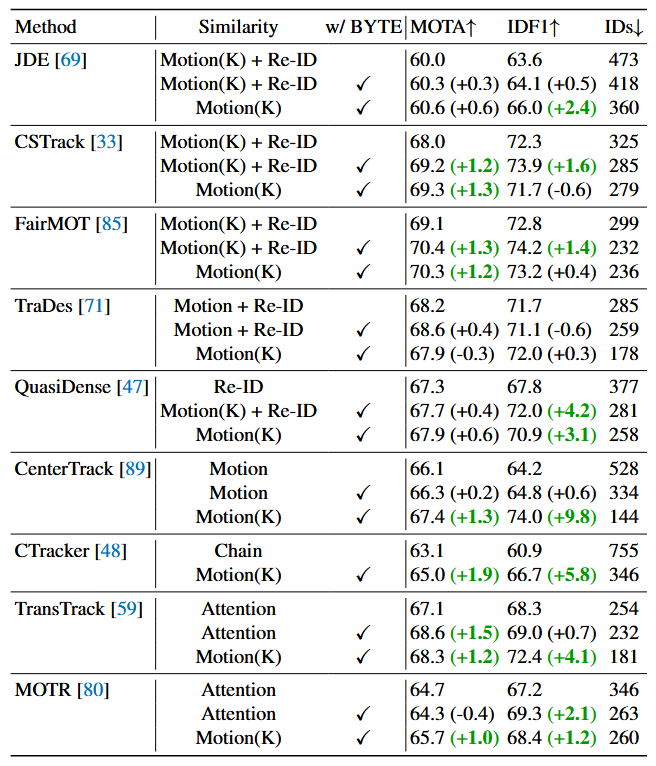
\includegraphics[width=0.8\textwidth]{images/BYTE/result1.png}
	\caption{在MOT17数据集上的结果}
	\label{btye_1}
\end{figure}


\section{论文学习}
数据关联的方法还有许多,本文的方法是基于SORT(DEEPSORT)的方法衍生而来,更偏向工程应用的一种方法。
数学上还有很多方法,例如最近邻、航迹分裂、01整数规则、联合概率数据关联(JPDA)和神经网络。
